\documentclass[a4paper, 10pt, french]{article}
% Préambule; packages qui peuvent être utiles
   \RequirePackage[T1]{fontenc}        % Ce package pourrit les pdf...
   \RequirePackage{babel,indentfirst}  % Pour les césures correctes,
                                       % et pour indenter au début de chaque paragraphe
   \RequirePackage[utf8]{inputenc}   % Pour pouvoir utiliser directement les accents
                                     % et autres caractères français
   % \RequirePackage{lmodern,tgpagella} % Police de caractères
   \textwidth 17cm \textheight 25cm \oddsidemargin -0.24cm % Définition taille de la page
   \evensidemargin -1.24cm \topskip 0cm \headheight -1.5cm % Définition des marges
   \RequirePackage{latexsym}                  % Symboles
   \RequirePackage{amsmath}                   % Symboles mathématiques
   \RequirePackage{tikz}   % Pour faire des schémas
   \RequirePackage{graphicx} % Pour inclure des images
   \RequirePackage{listings} % pour mettre des listings
   \usepackage{lmodern}
   %\usepackage{courier}
   \usepackage{graphicx}
% Fin Préambule; package qui peuvent être utiles

\title{Rapport de TP 4MMAOD : Génération d'ABR optimal}
\author{
ELOUATI Hossam (ISI$_1$)
\\ HAMOUMI Youness (ISI$_1$)
}

\begin{document}

\maketitle



%%%%%%%%%%%%%%%%%%%%%%%%%%%%%%%%%%%%%%%%%%%%%%

\textbf{Questions préliminaires : Équation de Bellman} \\
\\
\underline{Question 1:} Calcul de la somme $\sum_{l=i}^{j-1}p_l$ \\
\\
On note pour $i$ et $j$:
$$
\alpha(i,j) = \sum_{l=i}^{j-1}p_l
$$
On stocke les valeurs de $\alpha(i,j)$ dans un tableau bidimensionnel
 au lieu de calculer la valeur de $\alpha(i,j)$ chaque fois que l'on calcule
 $C(i,j)$ (dans ce cas, $\Theta(j-i)$ opérations d'additions seront nécessaires).
 Mieux vaut placer ces termes dans un tableau de $n^2$ éléments, et on retrouve la
 formule de récurrence suivante:
 $$
 \alpha(i,j) = \left\{
     \begin{array}{ll}
         p_{i} & \mbox{si } j=i+1 \\
         \alpha(i,j-1) + p_{j-1} & \mbox{si } 0 \leq i < j \leq n \\
         0 & \mbox{sinon.}
     \end{array}
 \right.
 $$
 Le calcul de chaque terme se fait alors avec $\Theta(1)$ opérations.
\\
\\
\underline{Question 2:} Espace mémoire et nombre d'opérations \\
\\
- Tableau pour stocker les valeurs de $C(i,j)$. Si une unité est une case du tableau,
alors, il faut $\Theta(n^2)$ en espace mémoire. \\
- Tableau pour stocker les valeurs de $\alpha(i,j)$. Donc, $\Theta(n^2)$. \\
Au total: l'espace mémoire est donc: $\Theta(n^2)$.
\\
Etant donné $i$ et $j$, on a besoin de 1 opérations pour calculer
$\alpha(i,j)$, de $\sum_{k=i}^{j}2$ pour calculer $C(i,j)$. Enfin, on a
besoin de $(j-i)$ comparaisons pour déterminer le $min$. \\
On obtient la somme suivante:
$$
T(n) = \sum_{j=1}^{n}\sum_{i=0}^{j-1}1+j-i+\sum_{k=i}^{j}2
$$
Par calcul direct on obtient que $T(n) = \Theta(n^3)$.
\\
\\
\underline{Question 3:} \\
\\
On a pour $i' \leq i \leq j \leq j'$, $\alpha(i,j) \leq \alpha(i',j')$.\\
De plus, $\alpha(i,j) + \alpha(i',j') = \alpha(i',j') + \alpha(i,j)$ et $\alpha(i,j) = \alpha(0,j)- \alpha(i,0)$.\\
Donc, on en déduit que pour: $i' \leq i \leq j \leq j'$, on a:$$ c(i,j) + c(i',j') \leq c(i',j)+c(i,j')$$
On pose à présent, $c^{k}(i,j) = \alpha(i,j)+c(i,k)+c(k+1,j)$ \\
On a: $r(i,j) = max(k \in [i,j-1] ; c^k(i,j) = c(i,j))$ = $max(k \in [i,j-1] ; \forall k', c^{k'}(i,j) \leq c^k(i,j))$\\
Comme $c(k+1, j-1) + c(k'+1,j) \leq c(k'+1, j-1) + c(k+1,j)$, on a: $$ c^k(i,j-1) + c^{k'}(i,j) \leq c^{k'}(i,j-1) + c^k(i,j) $$.
On obtient par conséquent que: $r(i,j-1) \leq r(i,j)$. \\
De même, on obtient $r(i,j) \leq r(i+1,j)$.\\
Avec cette restriction, le coût devient: $\Theta(n^2)$ et l'équation de Bellman devient:
$$
C(i,j) = \underset{r(i,j-1)\leq r \leq r(i+1,j)}{\min} C(i,r) + C(r+1,j) + \alpha(i,j)
$$
\section{Principe de notre  programme (1 point)}
{Notre programme se fait en deux étapes. Une première étape, itérative, permet de calculer le coût de recherche dans un arbre binanire de recherche
optimal. On effectue d'abord un calcul de coût pour tous les sous ABR. On stocke ces valeurs dans un tableau à deux dimensions \texttt{costs}.
La case \texttt{costs[i][j]} correspond au coût optimal du sous arbre \texttt{A(i,j)}. On utilisera également un tableau \texttt{roots}
pour mémoriser les valeurs des indices de racine pour chaque sous-arbre. Le remplissage de ces deux tableaux se fait de façon parallèle en se
basant sur l'équation de Bellman améliorée.
\\La deuxième étape, récursive, vient après avoir rempli le tableau \texttt{roots}, on extrait l'indice de la racine $r$ de l'arbre, soit \texttt{roots[0][nombre-elements]}, puis le même travail
se fait pour les deux sous arbres de racines respectives fils gauche et fils droite de l'élément $e_r$.
} 

%%%%%%%%%%%%%%%%%%%%%%%%%%%%%%%%%%%%%%%%%%%%%%
\section{Analyse du coût théorique (2 points)}


  \subsection{Nombre d'opérations en pire cas\,: }
    \paragraph{Partie itérative : Calcul du coût}
    {Dans la boule \texttt{for} sur \texttt{r}, on effectue au pire des cas deux additions et une comparaison.
    Ceci est traduit par la somme suivante: }
      $$T_{1}(n) = \sum_{i=0}^{n-1}\sum_{j=i+2}^{n}3(r_{i+1,j} - r_{i,j-1}+1) $$
      Par calcul direct on obtient:
      $$T_1(n) = \Theta(n^2)$$
    \paragraph{Partie récursive : Récupération de l'ABR optimal}
    {Pour la racine de l'ABR, on fait deux appels récursives si cette racine admet deux fils, sinon on effectue un seul appel.
    Pour les feuilles de l'ABR, on n'effectue aucun appel récursif. On conclut alors que le nombre d'appels récursifs est exactement
    le nombre d'éléments du dictionnaire, donc:
     $$T_{2}(n) = n$$}
    } 
  \subsection{Place mémoire requise\,: }
    {On suppose que l'unité de mémoire est la case occupée par un \texttt{int}. Pour notre programme, on a besoin de 5 tableaux: un tableau \texttt{probability} de taille ($n$) pour stocker les probabilités,
    un tableau \texttt{roots} de taille ($n(n+1)$), un tableau \texttt{sum-probabilities} de taille ($n(n+1)$) pour stocker les sommes de probabilités, un tableau \texttt{costs} de taille ($n(n+1)$) et le tableau
    \texttt{BSTtree} de taille ($2n$)}.
    \paragraph{Conclusion: }
    {La place mémoire requise est: $\Theta(n^2)$.}

  \subsection{Nombre de défauts de cache sur le modèle CO\,: }
    {On considère un cache de taille $Z$ et des lignes de cache de taille $L$. \\
    On se place dans le cas général où $Z << n$:}
    \paragraph{Défauts de cache engendrés par l'algorithme du calcul du coût optimal: \\ }
    {Pour chaque $i$, le calcul des éléments \texttt{costs[i][i+1]} engendre $2\frac{n}{L}$ défauts. Au total, le calcul de tous ces éléments
    engendre $2n\frac{n}{L}$.\\
    Pour chaque $i$ et $j$, le calcul de \texttt{costs[i][j]} charge la ligne \texttt{costs[i][:]} donc $\frac{n}{L}$ défauts de cache et la colonne \texttt{costs[:][j]}
    donc: $n$ défauts de cache. En prenant également en considération l'accès linéaire aux deux tableaux \texttt{sum-probabilities} et \texttt{roots}, on obtient la somme suivante:
    $$ Q(n,Z,L) = 2\frac{n^2}{L}+\sum_{i=0}^{n-1}\sum_{j=i+2}^{n}n+\frac{n}{L}+2 = \Theta(n^3)$$
    }
    \paragraph{Défauts de cache engendrés par l'algorithme de récupération de l'arbre optimal: \\ }
    {
    Pour chaque élément de l'arbre, on accède à 5 éléments. Vu que le nombre d'appels récursifs est $n$, on conclut que
    ce programme récursif engendre $5n$ défauts de cache, ce qui fait $\Theta(n)$.
    }




%%%%%%%%%%%%%%%%%%%%%%%%%%%%%%%%%%%%%%%%%%%%%%
\section{Compte rendu d'expérimentation (2 points)}
  \subsection{Conditions expérimentales}
     {

    \subsubsection{Description synthétique de la machine\,:} 
      {Les mesures de performances et de défauts de cache sont effectués sur une machine \texttt{DELL} portable, version \texttt{1.4.2}, système d'exploitation \texttt{Ubuntu}, processeur \texttt{Intel Core i5-8250U}, comportant un cache de \texttt{6144 KB} et
      une clock speed maximal de \texttt{3400 MHz}. Les mesures sont également effectuées au moment où seul le programme en question est en cours d'exécution et qu'aucun autre programme n'est lancé.
      } 

    \subsubsection{Méthode utilisée pour les mesures de temps\,: } 
      {En utilisant la fonction \texttt{clock()} de la bibliothèque \texttt{time.h}, on prélève un instant avant et après
      l'appel à la fonction \texttt{computing-BST}, chargé du calcul des coûts optimaux des dous arbres et de la construction
      de l'ABR optimal. La différence entre ces deux instants donne le temps d'exécution étant donné une valeur de $n$. La valeur de
      ce temps d'exécution est exprimée par l'unité de temps \texttt{CLOCKS}.
      }

  \subsection{Mesures expérimentales}
    {

    \begin{figure}[ht]
      \begin{center}
        \begin{tabular}{|l|r|r|r||}
          \hline
          \hline
                     & temps     & temps   & temps \\
                 & min       & max     & moyen \\
          \hline
          \hline
            benchmark1  &  31   &  85   &   64.6  \\
          \hline
            benchmark2  &  20   &  46   &  39.6   \\
          \hline
            benchmark3  &  25986  &  49885 & 31291.4    \\
          \hline
            benchmark4  &  86918   & 91254    & 88741.2    \\
          \hline
            benchmark5  &  193042   & 196391    & 194173.8   \\
          \hline
            benchmark6  &  559702   &  567199   & 563026.4    \\
          \hline
          \hline
        \end{tabular}
        \caption{Mesures des temps minimum, maximum et moyen de 5 exécutions pour les 6 benchmarks.}
        \label{table-temps}
      \end{center}
    \end{figure}
}
\subsection{Analyse des résultats expérimentaux}
{
\begin{center}
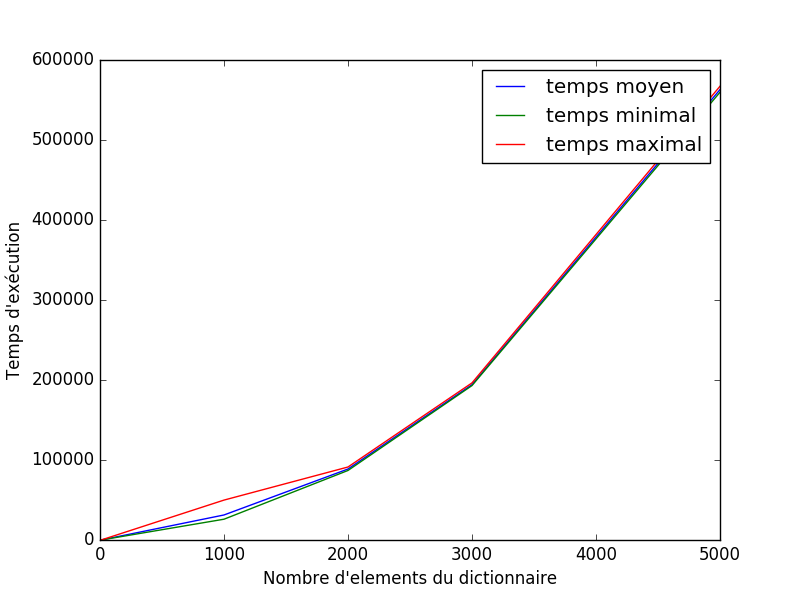
\includegraphics[width=10cm]{fi.png}
\end{center}
\begin{center}
\caption{FIGURE 2 - Temps d'exécutions en fonction du nombre des élements du dictionnaire}
\end{center}
Dans la figure 2, l'évolution de la courbe est plus ou moins lente. Cette évolution montre que le temps est quadratique par rapport au nombre d'éléments du dictionnaire, ce qui renforce le résultat obtenu dans la partie théorique. \\
\newline
Grâce à la commande \texttt{valgrind --tool=cachegrind ./ABR}, on calcule les défauts de cache engendrés par le programme pour chaque benchmark. On obtient la courbe suivante:
\begin{center}
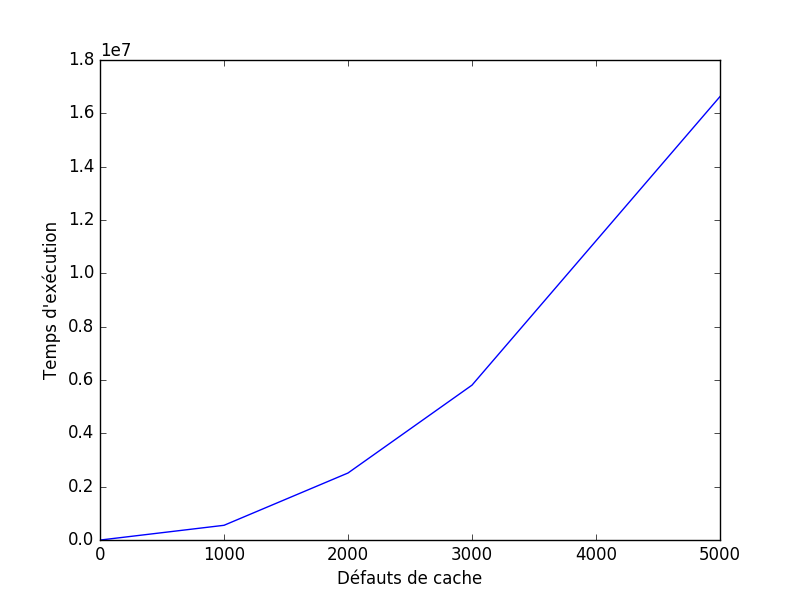
\includegraphics[width=10cm]{fig.png}
\end{center}
\begin{center}
\caption{FIGURE 3 - Défauts de cache en fonction du nombre des élements du dictionnaire}
\end{center}
}
Dans la figure 3, l'évolution de la courbe est considérablement rapide (atteint rapidement de très grandes valeurs). Ce qui montre que le nombre de défauts de cache est cubique par rapport au nombre d'éléments du dictionnaire (Résultat de l'analyse théorique).




\end{document}


%% Fin mise au format

